\section{Aula 5}

\subsection{Introdução}

No capítulo \ref{sec:4} vimos como funciona um sistema elétrico baseado apenas em unidades termelétricas. No entanto, um sistema elétrico real possui outras fontes como hidrelétricas e outras fontes renováveis. No caso Brasileiro, as hidrelétricas são até mais importantes do que as térmicas. Uma coisa que nós descobrimos, foi que o problema das térmicas pode ser resolvido de forma desacoplada, ou seja, resolvemos o problema para o despacho de hoje independentemente do problema de ontem e do de amanhã. 

Esta independência temporal não é verdadeira quando introduzimos hidrelétricas no sistema. O problema é que o custo marginal para gerar um megawatt hora de uma hidrelétrica é 0. Se mantemos o problema desacoplado no tempo, o resultado da otimização fará com que todo o reservatório da hidrelétrica seja utilizado de uma só vez, fazendo com que no futuro as térmicas mais caras sejam ligadas. 

Vamos começar com um exemplo bem simples para recapitular. Suponha um sistema unicamente térmico descrito pela figura \ref{fig:sist5}. Temos três unidades termelétricas que devem atender a uma demanda de 22MWh. A solução do problema é apresentada nos quadrados vermelhos. A primeira unidade gera 10MWh, a segunda gera 5MWh e a terceira gera 7MHw. 

\begin{figure}[H]
\begin{centering}
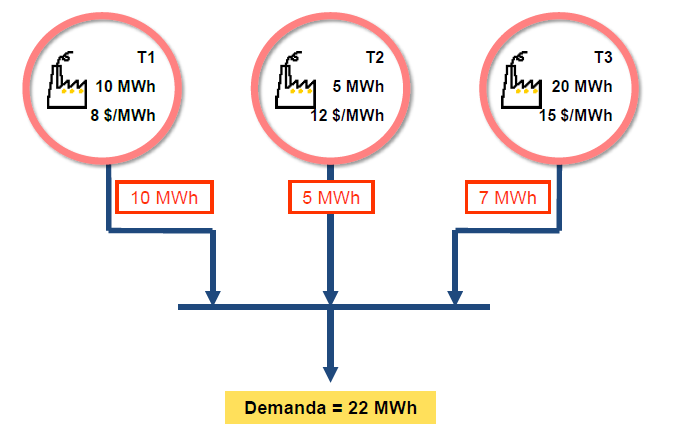
\includegraphics{aula5_1}\protect\caption{\label{fig:sist5} Pequeno sistema térmico}
\end{centering}
\end{figure}

Sabemos que o problema apresentado é a versão mais simples de um sistema termelétrico discutido no capítulo \ref{sec:4}. Ele é formulado com uma função objetivo que minimiza os custos do sistema sujeito à restrições de demanda e de capacidade de produção. 

\begin{align}
    & \underset{g\geq0}{\text{Min}} \hspace{1cm} 8g_1+12g_2+15g_3  \\
    & \text{s.a}  \hspace{2.2cm} g_1+g_2+g_3 \geq 22;  \\
    &             \hspace{2.65cm} g_1\leq 10, \\
    &             \hspace{2.65cm} g_2\leq 5. \\
    &             \hspace{2.65cm} g_3\leq 20. 
\end{align}

O sistema apresentado mostra bem aquilo que falamos anteriormente: não há nada que ligue a decisão hoje com a decisão em qualquer outro período de tempo. Vamos utilizar este mesmo sistema nos próximos exemplos para construir um modelo hidrotérmico.

\subsection{Sistemas hidrotérmicos}

Uma hidrelétrica é conhecida por ter um elevado custo de construção e um custo marginal muito próximo de zero. Isso é consequência direta do combustível utilizado, que no caso é a água. A água é de graça, e a hidrelétrica trabalha utilizando sua energia potencial. A capacidade de produção depende basicamente de dois fatores: a altura da queda d'água e a quantidade de água disponível. Portanto, é verdade que em muitos casos, usinas com reservatórios vazios geram pouco. A figura \ref{fig:hidro} exemplifica o funcionamento de uma hidrelétrica. Em linhas gerais, as hidrelétrica possuem uma represa que assegura um reservatório de água, a água passa por uma turbina que está acoplada a um gerador. Se por acaso o reservatório estiver muito cheio, chegando nos limites da represa, a água é vertida (jogada fora).  

\begin{figure}[H]
\begin{centering}
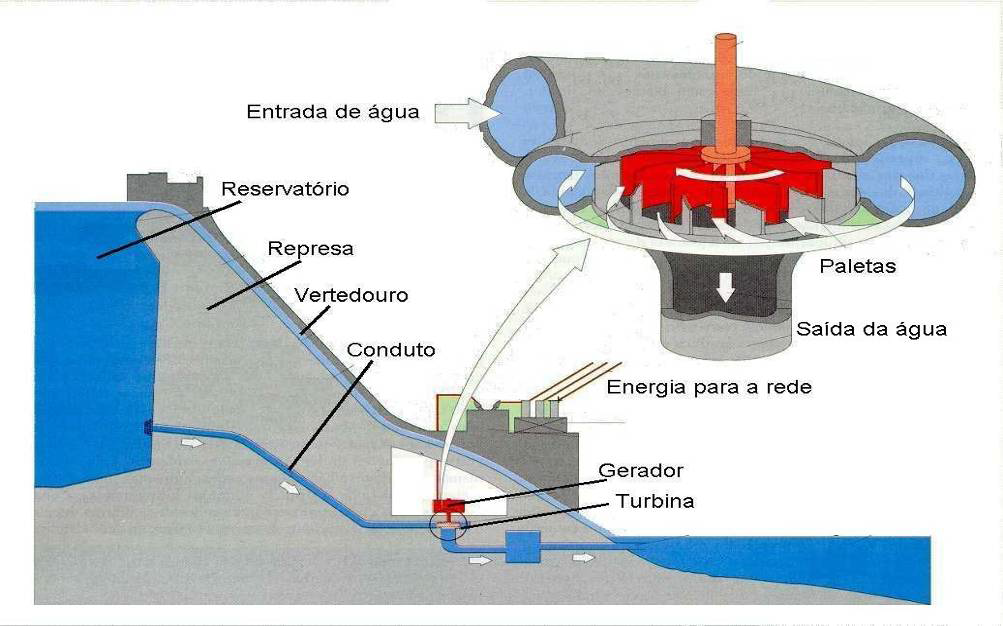
\includegraphics[scale=0.6]{aula5_2}\protect\caption{\label{fig:hidro} Geração Hidrelétrica}
\end{centering}
\end{figure}

Um gerador hidrelétrico tem uma série de nova variáveis em questão. Como mencionamos anteriormente, a geração em MWh depende de uma relação entre a vazão turbinada em $m^2/s$ e pela altura de queda líquida em metros. As relações entre estas variáveis é não linear e complexa. Além disso, temos as variáveis do reservatório como volume máximo e volume mínimo (em usinas fio d'água o volume máximo é igual ao mínimo). A topologia, a capacidade de turbinamento, restrições de navegação e segurança das populações locais também devem ser consideradas. Finalmente, a dinâmica de uma usina hidrelétrica depende das usinas que estão a \textbf{montante}\footnote{As usinas que vem abaixo estão a jusante da usina em questão.} dela, ou seja, daquelas que estão acima dela no curso do rio. Em resumo, temos um \textbf{balanço hidráulico} que deve entrar no modelo de otimização, apresentado na Figura \ref{fig:balhid}. 

\begin{figure}[H]
\begin{centering}
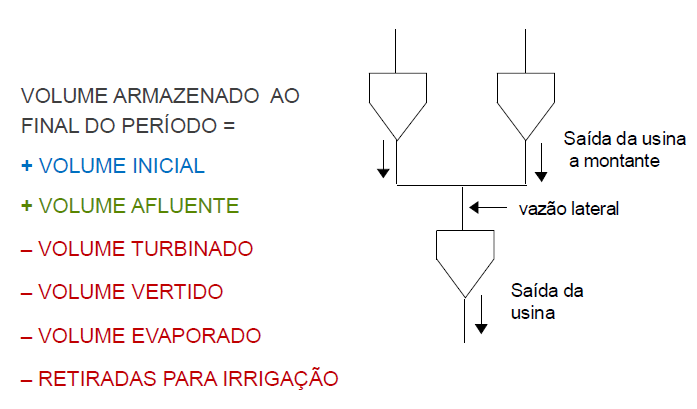
\includegraphics[scale=0.9]{aula5_3}\protect\caption{\label{fig:balhid} Balanço Hidráulico}
\end{centering}
\end{figure}

No início do período temos um volume inicial de água. Além disso, temos o volume afluente, que é a água que chega ao reservatório. Devemos considerar também a água que sai de diversas formas, são elas: o volume turbinado, o volume vertido (jogado fora), o volume perdido para evaporação e retiradas de água para irrigação e outras atividades. O resultado desta conta resultará no volume final do reservatório, que será também o volume inicial do próximo período. Já começa a ficar claro porque o problema hidrelétrico não pode ser resolvido de forma desacoplada temporalmente. Existe uma variável que conecta os diversos períodos, no caso, o volume do reservatório. 

\begin{figure}[H]
\begin{centering}
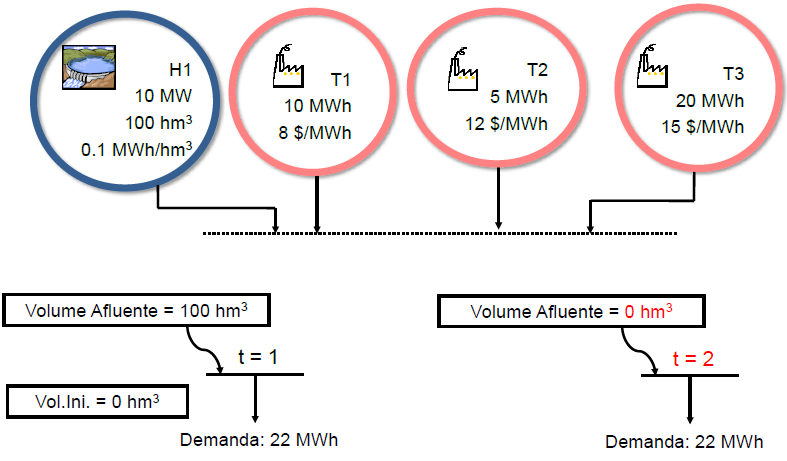
\includegraphics[scale=0.77]{aula5_4}\protect\caption{\label{fig:hdrotermico1}Pequeno sistema hidrotérmico}
\end{centering}
\end{figure}

Vamos voltar para o exemplo anterior. A Figura \ref{fig:hdrotermico1} mostra o sistema térmico da sessão anterior com mais uma usina hidrelétrica. Além disso, agora o operador precisa resolver o problema para dois estágios, $t=1$ e $t=2$. O reservatório começa vazio, mas recebe um volume de 100 hectômetros cúbicos ($hm^3$) em $t=1$. Em $t=2$ o reservatório não recebe água. A demanda nos dois períodos é igual a 22MWh. Como devemos atacar este problema? A primeira possibilidade é utilizar todo o reservatório no período 1, e no período 2 geramos apenas com as térmicas. Assim, a hidrelétrica, que gera 0.1 MHw por hectômetro cúbico irá gerar 10Mhw, a unidade termelétrica mais barata irá gerar 10MHw e a termelétrica seguinte gerará 2MHw. O custo no período 1 seria de $\$104$. No período dois teríamos que usar apenas as térmicas, e o resultado seria o mesmo do exemplo da sessão anterior, com um custo de $\$245$. O custo total seria então $\$349$. Esta solução é ótima? Antes de responder esta questão, vamos montar o problema completo para os dois estágios. {\color[rgb]{1,0,0} This text will appear red-colored} 

\begin{align}
    & \underset{g\geq0}{\text{Min}} \hspace{1cm} 8g_{1,1}+12g_{2,1}+15g_{3,1}+8g_{1,2}+12g_{2,2}+15g_{3,2}  \\
    & \text{s.a}  \hspace{2.2cm} g_1+g_2+g_3+gh_1 \geq 22;  \\
    &             \hspace{2.65cm} vol_0=100\\
    &             \hspace{2.65cm} {\color[rgb]{1,0,0}vol_1}= vol_0+0-gh_1\\
    &             \hspace{2.65cm} g_{1,1}\leq 10, \\
    &             \hspace{2.65cm} g_{2,1}\leq 5. \\
    &             \hspace{2.65cm} g_{3,1}\leq 20. \\
    &             \hspace{2.65cm} g_{1,2}\leq 10, \\
    &             \hspace{2.65cm} g_{2,2}\leq 5. \\
    &             \hspace{2.65cm} g_{3,2}\leq 20. \\
    &             \hspace{2.65cm} gh_1\leq 0.1\times100=10\\
    &             \hspace{2.65cm} gh_2\leq 0.1\times {\color[rgb]{1,0,0}vol_1}
\end{align}


A primeira coisa que podemos notar é que o problema cresceu bastante com a inclusão de uma hidrelétrica e mais um período. A função objetivo agora inclui os custos das termelétricas em $t=1$ e $t=2$, no entanto, os custos das hidrelétrica não aparecem. Isto acontece porque para gerar energia a hidrelétrica não tem custo. Uma coisa é muito importante, se não fosse pela variável $vol_1$ (que por convenção representa quanto de água temos ao final do período 1 ou início do período 2), que marcamos em vermelho, o problema hidrotérmico poderia ser desacoplado no tempo como aquele exclusivamente térmico. Esta variável é aquela que informa como o reservatório chega no início do período 2. Como a geração hidrelétrica no período 2 está limitada a $vol_1$, então os dois períodos passam a estar conectados. 

Vamos retomar a busca pelo ótimo. Será que nossa solução de utilizar toda a água é a melhor possível? Sabemos que no total, considerando $t=1$ e $t=2$, podemos gerar 10MHw de energia térmica. A tabela \ref{tab:5.1} mostra o que acontece com o custo total quando distribuímos a geração hidrelétrica de formas diferentes no tempo. Pela tabela vemos que o ótimo não é fazer aquilo que foi nossa primeira tentativa, ou seja, usar toda a energia hidrelétrica de uma vez em $t=1$. O ótimo estará no ponto em que geramos entre 4 e 6 MHw de energia hidrelétrica em $t=1$. Para qualquer uma destas escolhas, utilizaremos exatamente 4 MHw da usina mais cara somando os dois períodos. É justamente aí que está toda a questão, quando dividimos a geração hidrelétrica entre os períodos acabamos tendo que ligar menos as térmicas mais caras quando consideramos o horizonte como um todo. Consequentemente, o custo total é menor.  

\begin{table}[h]
\caption{Custos de geração}
\label{tab:5.1}
\centering
\begin{tabular}{ccccccc}
\hline
\multicolumn{4}{c}{Decisão na etapa 1} & Custo na etapa 1 & Custo na etapa 2 & Custo Total \\ \hline
Hidro      & T1      & T2     & T3     & CT1              & CT2              & CT1$+$CT2   \\ \hline
10         & 10      & 2      & 0      & 104              & 245              & 349         \\
8          & 10      & 4      & 0      & 128              & 215              & 343         \\
6          & 10      & 5      & 1      & 155              & 185              & 340         \\
4          & 10      & 5      & 3      & 185              & 155              & 340         \\
2          & 10      & 5      & 5      & 215              & 128              & 343         \\
0          & 10      & 5      & 7      & 245              & 104              & 349         \\ \hline
\end{tabular}
\end{table}


Uma forma interessante de interpretar o problema apresentado é separando o custo em duas funções, a \textbf{Função de Custo Imediato} (FCI)
 e a \textbf{Função de Custo Futuro} (FCF). A FCF considera todos os períodos a frente, mesmo se o problema tiver mais de dois períodos. Desejamos então minimizar a soma do FCF e do FCI. 

\subsubsection{Função de Custo Futuro e Função de Custo Imediato}

A função de custo futuro e a função de custo imediato nos permite separar o problema em duas partes. A parte imediata é o problema de otimização no período atual, e a parte futura é uma função que criamos para representar os custos futuros. Veremos mais adiante que esta divisão nos permite resolver o problema de trás para frente em pequenos probleminhas mais simples. 

\begin{figure}[H]
\begin{centering}
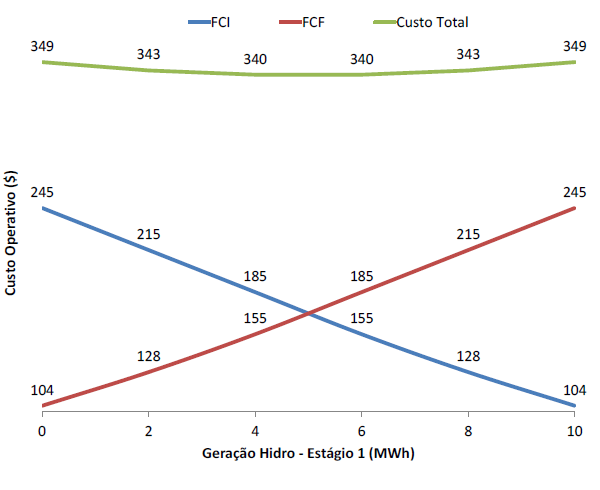
\includegraphics[scale=0.6]{aula5_5}\protect\caption{\label{fig:fcifcf} FCI e FCF}
\end{centering}
\end{figure}


A figura \ref{fig:fcifcf} passa a intuição do que estamos mostrando. O gráfico inferior mostra o que acontece com o custo em cada um dos períodos quando alteramos a geração no período 1. Observe que se exaurimos a hidrelétrica neste período, temos custos muito baixos, mas teremos que pagar a conta no futuro devido à falta de água. Assim, se somamos estes dois custos temos a curva do custo total, apresentada na parte superior da figura. Além disso, a Figura \ref{fig:fcifcf1} mostra que a partir desta separação dos custos podemos obter o \textbf{valor da água}, que é o quanto alguém pagaria por uma unidade a mais deste recurso. Em linhas gerais, o valor da água nos mostra o quanto ganhamos com a redução na geração térmica no período dois obtida através de uma economia de água no período um. Voltando ao exemplo anterior, suponha que chegamos ao período 2 sem água, ou seja, utilizamos tudo no período 1. Sabemos que um hectômetro cúbico de água a mais gera 0.1MWh extra de energia. Como o custo marginal de operação da térmica mais cara, que estará ligada neste caso, é de $\$15$ por MWh, então $1Hm^3$ a mais de água nos gera uma economia de $\$1.5$. Este será o valor da água neste caso. Como exercício, tente calcular o valor da água quando chegamos ao período 2 com volumes diferentes de água. 

\begin{figure}[H]
\begin{centering}
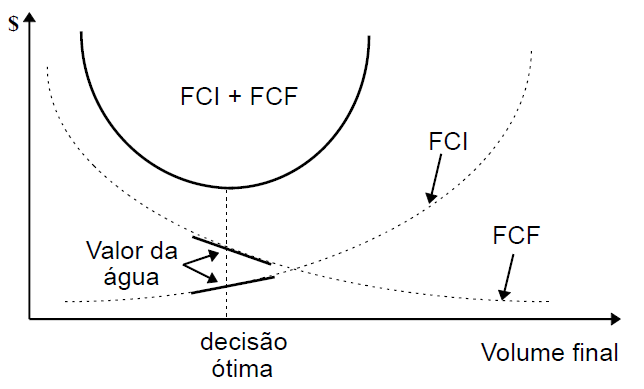
\includegraphics[scale=0.6]{aula5_6}\protect\caption{\label{fig:fcifcf1} FCI, FCF e o Valor da Água} 
\end{centering}
\end{figure}

Podemos dizer agora que a água possui um custo de oportunidade, e que usa-la agora resultará em custos mais altos no futuro. Isso deve ser levado em conta na hora de resolver o problema do despacho hidrotérmico. A solução ótima sera aquela que minimiza a soma $FCI+FCF$, fazendo com que parte da água seja economizada no intuito de reduzir os custos no futuro. O despacho ótimo é obtido quando o valor da água agora é igual à seu valor no futuro. Imagine que a água valha mais agora, então vale a pena utilizar um pouco mais até igualar aos custos futuros. No caso contrário, em que a água vale mais lá na frente, então economizamos agora para reduzir os custos futuros. Podemos agora escrever o problema do despacho hidrotérmico em sua forma mais geral:

\begin{align}
    & \underset{g\geq0}{\text{Min}} \hspace{1cm} \sum_{j=1}^J c_jg_{t,j}+FCF(v_{t+1})  \\
    & \text{s.a}  \hspace{2.2cm} v_{t+1}=v_t+a_t-u_t-s_t   \\
    &             \hspace{2.65cm} v_{t+1}\leq \bar{v} \\
    &             \hspace{2.65cm} u_t\leq \bar{u} \\
    &             \hspace{2.65cm} \text{Restrições das térmicas}
\end{align}

onde, $c_j$ representa o custo do MHw da térmica $j$, $g_{t,j}$ é a geração da térmica $j$ no tempo $t$, $v_t$ é o volume de água que chega no início do tempo $t$, $a_t$ é a água que chega ao reservatório devido a fatores exógenos, $u_t$ é o volume turbinado e $s_t$ é o volume vertido. 

\subsection{Incerteza na Vazão}

Nosso modelo de despacho hidrotérmico ainda não está completo. Até este momento não tratamos de incerteza, mas na vida real, não sabemos a quantidade de água que teremos a nossa disposição no futuro. Claro, podemos ter uma previsão, mas nunca teremos certeza. Quanto temos incerteza sobre o futuro dizemos que o problema de otimização se tornou \textbf{estocástico}. Uma forma de modelar a incerteza é por meio de cenários, ou seja, adotamos um critério para construir várias possíveis realizações do futuro e dizemos para o modelo minimizar, por exemplo, o custo médio levando em conta todas as possibilidades. Uma forma de representar estes cenários é por meio de uma árvore como na figura \ref{fig:tree1}. Por convenção, s quadrados verdes são \textbf{nós de decisão} e os círculos vermelhos são \textbf{nós de incerteza}, os triângulos azuis mostram o fim da árvore. Quando tomamo a decisão de utilizar a água, ainda não sabemos o que vai acontecer, portanto, o nó de decisão vem antes dos nós de incerteza. Neste exemplo, existem dois possíveis cenários: úmidos e secos. Se o operador decide utilizar os reservatórios e se depara com um cenário seco, por exemplo, ele estará em uma situação de defict, e terá que arcar com custos mais elevados na operação do sistema devido à utilização de térmicas mais caras. 



\begin{figure}[H]
\begin{centering}
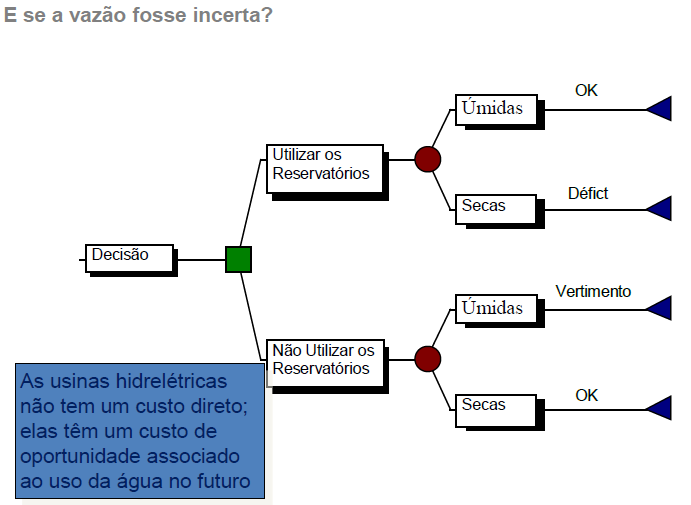
\includegraphics[scale=0.7]{aula5_7}\protect\caption{\label{fig:tree1} Árvore de decisão sobre incerteza na vasão} 
\end{centering}
\end{figure}

As árvores de decisão possuem mais uma informação, que diz respeito a probabilidade de ocorrência de cada cenário. Ou seja, em cada nó de incerteza devemos considerar qual a probabilidade de cada cenário ocorrer. Assim, se desejamos minimizar o custo médio, devemos considerar uma função objetivo que contenha o custo presente, que é determinístico, mais o custo futuro, que é estocástico. Ela irá minimizar a soma do primeiro com a média do segundo. O problema desta abordagem, é que se consideramos um número grande de cenários em um período de tempo muito longo, o problema cresce de forma exponencial e resolve-lo passa a ter um custo computacional muito alto. 

\subsubsection{Abordagem da árvore por estados: Programação Dinâmica Estocástica (PDE)}

Uma forma alternativa e mesmo custosa de resolver o problema é utilizando a abordagem de estados na árvore. Assim, um problema muito grande pode ser decomposto em problemas menores que enumeram a árvore de forma implícita. Basicamente, definimos o problema no período $t$ assumindo vários estado do sistema no início de $t$. Por exemplo, podemo dividir o reservatório em níveis de $0\%$, $10\%$ até $100\%$, assim resolvemos o problema para todos estes níveis e temos um esboço da função de custos do tempo $t$, que poderá ser utilizada como FCF no tempo $t+1$. 

Vamos construir o problema. Em primeiro lugar, devemos levar em conta que a abordagem de estados deve ser resolvida do último período para o primeiro, então vamos para o problema no tempo $T$. No tempo $T$ o mundo acaba, então não existe $T+1$, portanto o problema será:


\begin{align}
    & \underset{g\geq0}{\text{Min}} \hspace{1cm} \sum_{j=1}^J c_jg_{T,j}  \\
    & \text{s.a}  \hspace{2.2cm} v_{T+1}=v_T+a_T-u_T-s_T   \\
    &             \hspace{2.65cm} v_{T+1}\leq \bar{v} \\
    &             \hspace{2.65cm} u_T\leq \bar{u} \\
    &             \hspace{2.65cm} \text{Restrições das térmicas}
\end{align}

Note que utilizamos $v_{T+1}$ apenas para manter a restrição da capacidade do reservatório, o tempo $T+1$ não existe no problema. Vamos agora utilizar os estados do reservatório variando de $0\%$ a $100\%$ de $10\%$ em $10\%$. Teremos algo como mostrado na Figura \ref{fig:fcfsp}.

\begin{figure}[H]
\begin{centering}
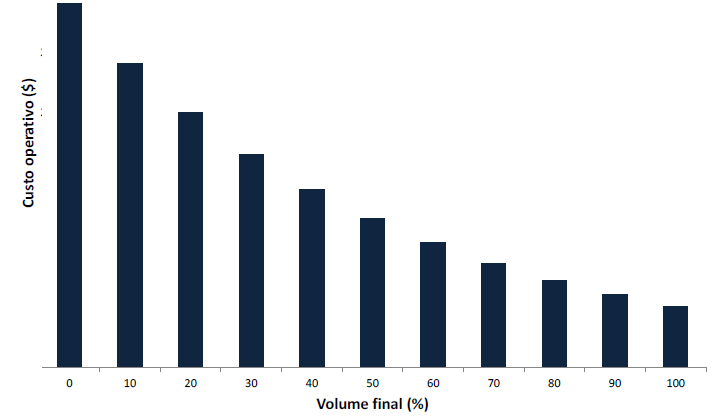
\includegraphics[scale=0.7]{aula5_8}\protect\caption{\label{fig:fcfsp} Custo em $T$ como função do volume de água} 
\end{centering}
\end{figure}

Observe que se interpolamos as barras da Figura \ref{fig:fcfsp} temos uma função linear por parte que representa o custo em $T$. Além disso, sabemos que uma função deste tipo pode ser colocada dentro de um problema de otimização linear. Portanto, acabamos de construir a FCF que será utilizada no problema em $T-1$ representando o tempo $T$. Vamos então para o problema em $T-1$:

\begin{align}
    & \underset{g\geq0}{\text{Min}} \hspace{1cm} \sum_{j=1}^J c_jg_{T-1,j}+FCF(v_T)  \\
    & \text{s.a}  \hspace{2.2cm} v_{T}=v_{T-1}+a_{T-1}-u_{T-1}-s_{T-1}   \\
    &             \hspace{2.65cm} v_{T}\leq \bar{v} \\
    &             \hspace{2.65cm} u_{T-1}\leq \bar{u} \\
    &             \hspace{2.65cm} \text{Restrições das térmicas}
\end{align}


Agora devemos resolver o problema acima para todos os estados do reservatório em $T-1$ e teremos a FCF para utilizar no problema to tempo $T-2$. Se fizermos este procedimento até $T=1$, teremos uma solução para o problema completo que foi dividida em vários probleminhas. O problema apresentado aqui ainda está simplificado. Devemos nos lembrado do capítulo \ref{seq:4} que nos ensinou que existem outras restrições na operação do sistema, como por exemplo as linhas de transmissão. Estas restrições devem ser considerada na modelagem que apresentamos neste capítulo. 

\subsection{Programação Dinâmica Dual Estocástica}

Imagine que em um sistema elétrico de verdade podemos ter centenas de hidrelétricas. O que aconteceria com a programação dinâmica estocástica nesse caso? O problema cresceria de forma absurda e logo se tornaria inviável. Isto ocorre porque se consideramos vária hidrelétricas temos que considerar todos os estados de todas as hidrelétricas. Com duas usinas com 10 estados cada uma, teríamos um total de 100 estados para o sistema. Com 60 hidrelétrica, seriam $10^60$ estados. 

A programação dinâmica dual estocástica (PDDE) é uma boa alternativa quando o número de reservatórios é muito grande. Ao invés de calcularmos o custo futuro para todos os estágios, calculamos apenas para alguns. Lembre-se que a FCF é uma função linear por partes convexa, ou seja, ela é formada por vários segmentos de retas. Na PDDE utilizamos as variáveis duais do problema como coeficientes destes seguimentos. A inclinação de cada seguimento será dada pelo valor da água que discutimos anteriormente. 

A PDDE é um método iterativo de construção de aproximações da FCF em torno de pontos interessantes, ou seja, o mesmo procedimento é feito varias vezes para melhorar nosso conhecimento da função. Esses pontos interessantes são obtidos dentro do próprio modelo através de uma simulação de Monte Carlo. Devemos também adotar um critério de convergência, pois como se trata de um algorítimo, o computador deve saber quando parar. O problema de PDDE pode ser dividido em duas partes:

\begin{itemize}
\item Fase Foward (Simulação): Gera os pontos interessantes de armazenamento dos reservatórios em cada etapa considerando as aproximações da FCF já construídas em iterações anteriores.
\item Fase Backward (Recursão): Adiciona novos segmentos de reta nas aproximações da FCF de cada etapa obtidos em torno dos pontos interessantes de armazenamento gerados na fase foward. 
\end{itemize}

\todo{Tche, essa parte tem que completar com a aula 6 do Street.}

\subsection{Outras características do despacho hidrotérmico}

Nesta sessão nós vamos recapitular algumas características dos sistemas hidrotérmicos que já foram mencionadas e também apresentaremos algumas novidades. A primeira coisa que aprendemos é que os sistemas hidrotérmicos são acoplados no tempo pelos reservatórios. Portanto, devemos considerar a disponibilidade futura de água para tomar nossa decisão agora. Além disso, não sabemos quais são as afluências futuras, conhecemos apenas suas distribuições de probabilidade. Com tudo que foi estudado até agora, já podemos perceber que existe uma troca no sistema hidrotérmico entre confiabilidade e custo. Se colocamos nosso sistema $100\%$ nas térmicas temos uma confiabilidade muito alta, pois existem poucas incertezas na operação térmica que podem ser controladas com maior facilidade. Conforme vamos introduzindo hidrelétricas e colocando nosso sistema dependente delas, a confiabilidade tende a ser menor. Isso se deve ao fato de que a quantidade de incertezas passa a ser muito maior, e a possibilidade de erros que podem prejudicar o suprimento de energia é maior. 

\subsubsection{Modelagem de afluências}

Existe uma característica das afluências que não foi considerada até aqui: ela é \textbf{autocorrelacionada} no tempo. Em outras palavras, a afluência de hoje tem uma correlação com a de ontem. Além disso, existe também uma dependências espacial das afluências quando levamos em conta bacias hidrográficas. Esses fatores são modelados via séries temporais. Suponha que temos uma série de dados de um reservatório em vários períodos. Podemos considerar esta série como uma realização de um processo estocástico e utiliza-la para tentar construir outras realizações possíveis via simulação de Monte Carlo. Estas séries geradas são chamadas séries sintéticas, e elas devem ter algumas características que mantém sua semelhança com a série histórica original. Em outras palavras, alguns parâmetros chave como média, desvio padrão, correlações, dependências temporais e espaciais e estacionariedade devem ser preservados. 


\begin{figure}[H]
\begin{centering}
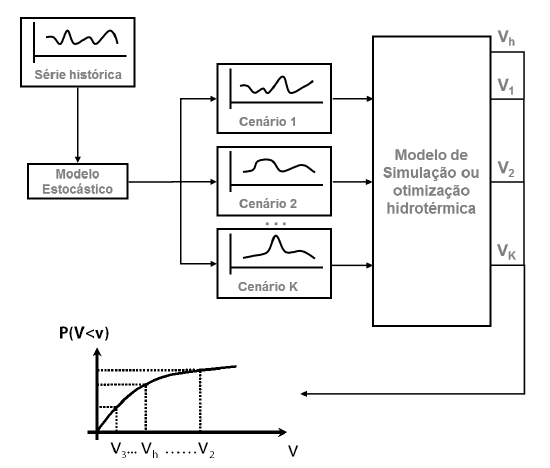
\includegraphics[scale=0.7]{aula5_9}\protect\caption{\label{fig:aflu1} Etapas da modelagem da afluência} 
\end{centering}
\end{figure}

A Figura \ref{fig:aflu1} mostra as etapas da modelagem da afluência e sua utilização nos modelos que otimização. Partimos de uma série histórica na qual estabelecemos um processo estocástico. Utilizamos este processo combinado com simulação de Monte Carlo para gerar inúmeros cenários que são as séries sintéticas. Estas séries sintéticas entrarão no nosso modelo de otimização ou de simulação. A questão é: qual modelo utilizamos para modelar a série histórica? Um modelo que se ajusta bem a este tipo de problema é o \textit{periodic autorregressive model} (PAR(p)). Neste modelo, a afluência no período $t$ depende das $p$ afluências anteriores. Além disso, existe uma estrutura periódica que faz com que o parâmetro $p$ dependa de em qual mês estamos.


\subsubsection{Custos de interrupção}

Já vimos nos capítulos anteriores que pode acontecê de não ser possível para o sistema elétrico suprir toda a demanda por energia em algum período de tempo. Tratamos esta situação colocando mais uma variável no modelo de otimização que diz respeito ao custo de interrupção do sistema. Esta variável é semelhante à incluir mais uma termelétrica que tem um custo mais alto que todas as demais e pode gerar energia infinita. Este procedimento é adotado pelo sistema elétrico brasileiro. Ademais, discutimos também o \textit{tradeoff} entre confiabilidade e custo. Se utilizamos um sistema exclusivamente hidrelétrico ficamos expostos a grandes riscos que não podem ser controlados com facilidade. Lembre-se que a partir do momento que nosso problema se tornou estocástico, nosso objetivo passou a ser minimizar a média ou o valor esperados dos custos levando em conta os possíveis cenários. O problema  de minimizar a média esta no fato dela ser uma medida \textbf{neutra ao risco}, ou seja, ela é incapaz de diferenciar entre duas soluções com o mesmo custo mas médio mas com probabilidades de interrupção do fornecimento de energia completamente diferentes. Não é isso que queremos, queremos uma medida que entre duas soluções de mesmo custo médio, escolha aquela que tem o menor risco. 

No dia 24 de julho de 2013 ficou estabelecido que o mecanismo de aversão ao risco utilizado no sistema elétrico brasileiro será o \textit{Conditional Value at Risk} (CVaR). Além de considerar a média, a introdução do CVaR faz com que o modelo considere também a média nos piores cenários na tomada de decisão. 


\begin{figure}[H]
\begin{centering}
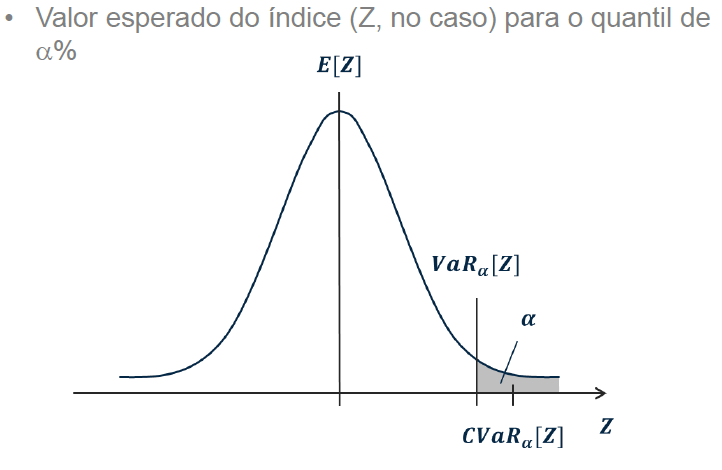
\includegraphics[scale=0.7]{aula5_10}\protect\caption{\label{fig:cvar1} Representação gráfica do CVaR} 
\end{centering}
\end{figure}

A Figura \ref{fig:cvar1} mostra uma representação gráfica bem intuitiva do CVaR. A figura mostra uma distribuição de probabilidade de custos com a média igual a $E[Z]$. O $CVaR_\alpha[Z]$ pode ser visto como a média nos $100\times \alpha \%$ piores cenários, que são representados pela área sombreada da figura. O CVaR pode ser introduzido no problema de otimização de duas formas: 1) adicionando uma restrição que coloca um teto para seu valor, ou seja, o CVaR não pode passar de $X$; 2) colocando o CVaR na função objetivo e criando uma ponderação entre a média e o CVaR. Esta segunda forma é aquela utilizada no sistema brasileiro, nela o parâmetro $\alpha$ é fixo e escolhido pelo usuário. Além disso, existe um parâmetro $\lambda$ também escolhido pelo usuário que define o peso dado para a média e o peso dado para o CVaR. A função objetivo que desejamos minimizar passa a ter a seguinte forma:

\begin{equation}
\min (1-\lambda)E(CO) + \lambda CVaR(CO)
\end{equation}

onde $CO$ é o custo operacional do sistema. Quanto maior o $\lambda$ mais o peso que estamos dando para o CVaR, e consequentemente, maior a aversão ao risco do modelo e maior a segurança do suprimento de energia. Entretanto, se colocamos lambda muito grande acabamos aumentando demais os custos. No Brasil os valores de $\alpha$ e $\lambda$ utilizados são $5\%$ e $25\%$. 

\subsubsection{Como é feito no Brasil}

No Brasil o planejamento e operação do sistema é feito utilizando três modelos, cada um considerando um horizonte de tempo. O NEWAVE possui um horizonte de tempo superior a 10 anos e é calculado mensalmente, este modelo é importante na construção do preço de liquidação de diferenças (PLD). O DECOMP tem o horizonte de um ano e é calculado semanalmente e o DESSEM tem o horizonte de uma semana e é calculado de hora em hora para operações de ajuste de curtíssimo prazo. O DECOMP também faz parte da construção do PLD. 



